\newpage 

\section*{Recommendations}

After the analysis, the government and the Central Bank should adopt a comprehensive strategy to 
stabilize the \textbf{\textcolor{teal}{financial sector}}, rebuild investor confidence, and promote 
long-term economic resilience in Macaronia. The following recommendations focus on enhancing
\textbf{\textcolor{teal}{monetary policy}}, strengthening financial stability, ensuring 
\textbf{\textcolor{teal}{exchange rate steadiness}}, and supporting vulnerable populations. 

\subsection*{Adjusting Monetary Policy to Help Balance Inflation \& Liquidity}

\begin{figure}[h]     
     \centering
     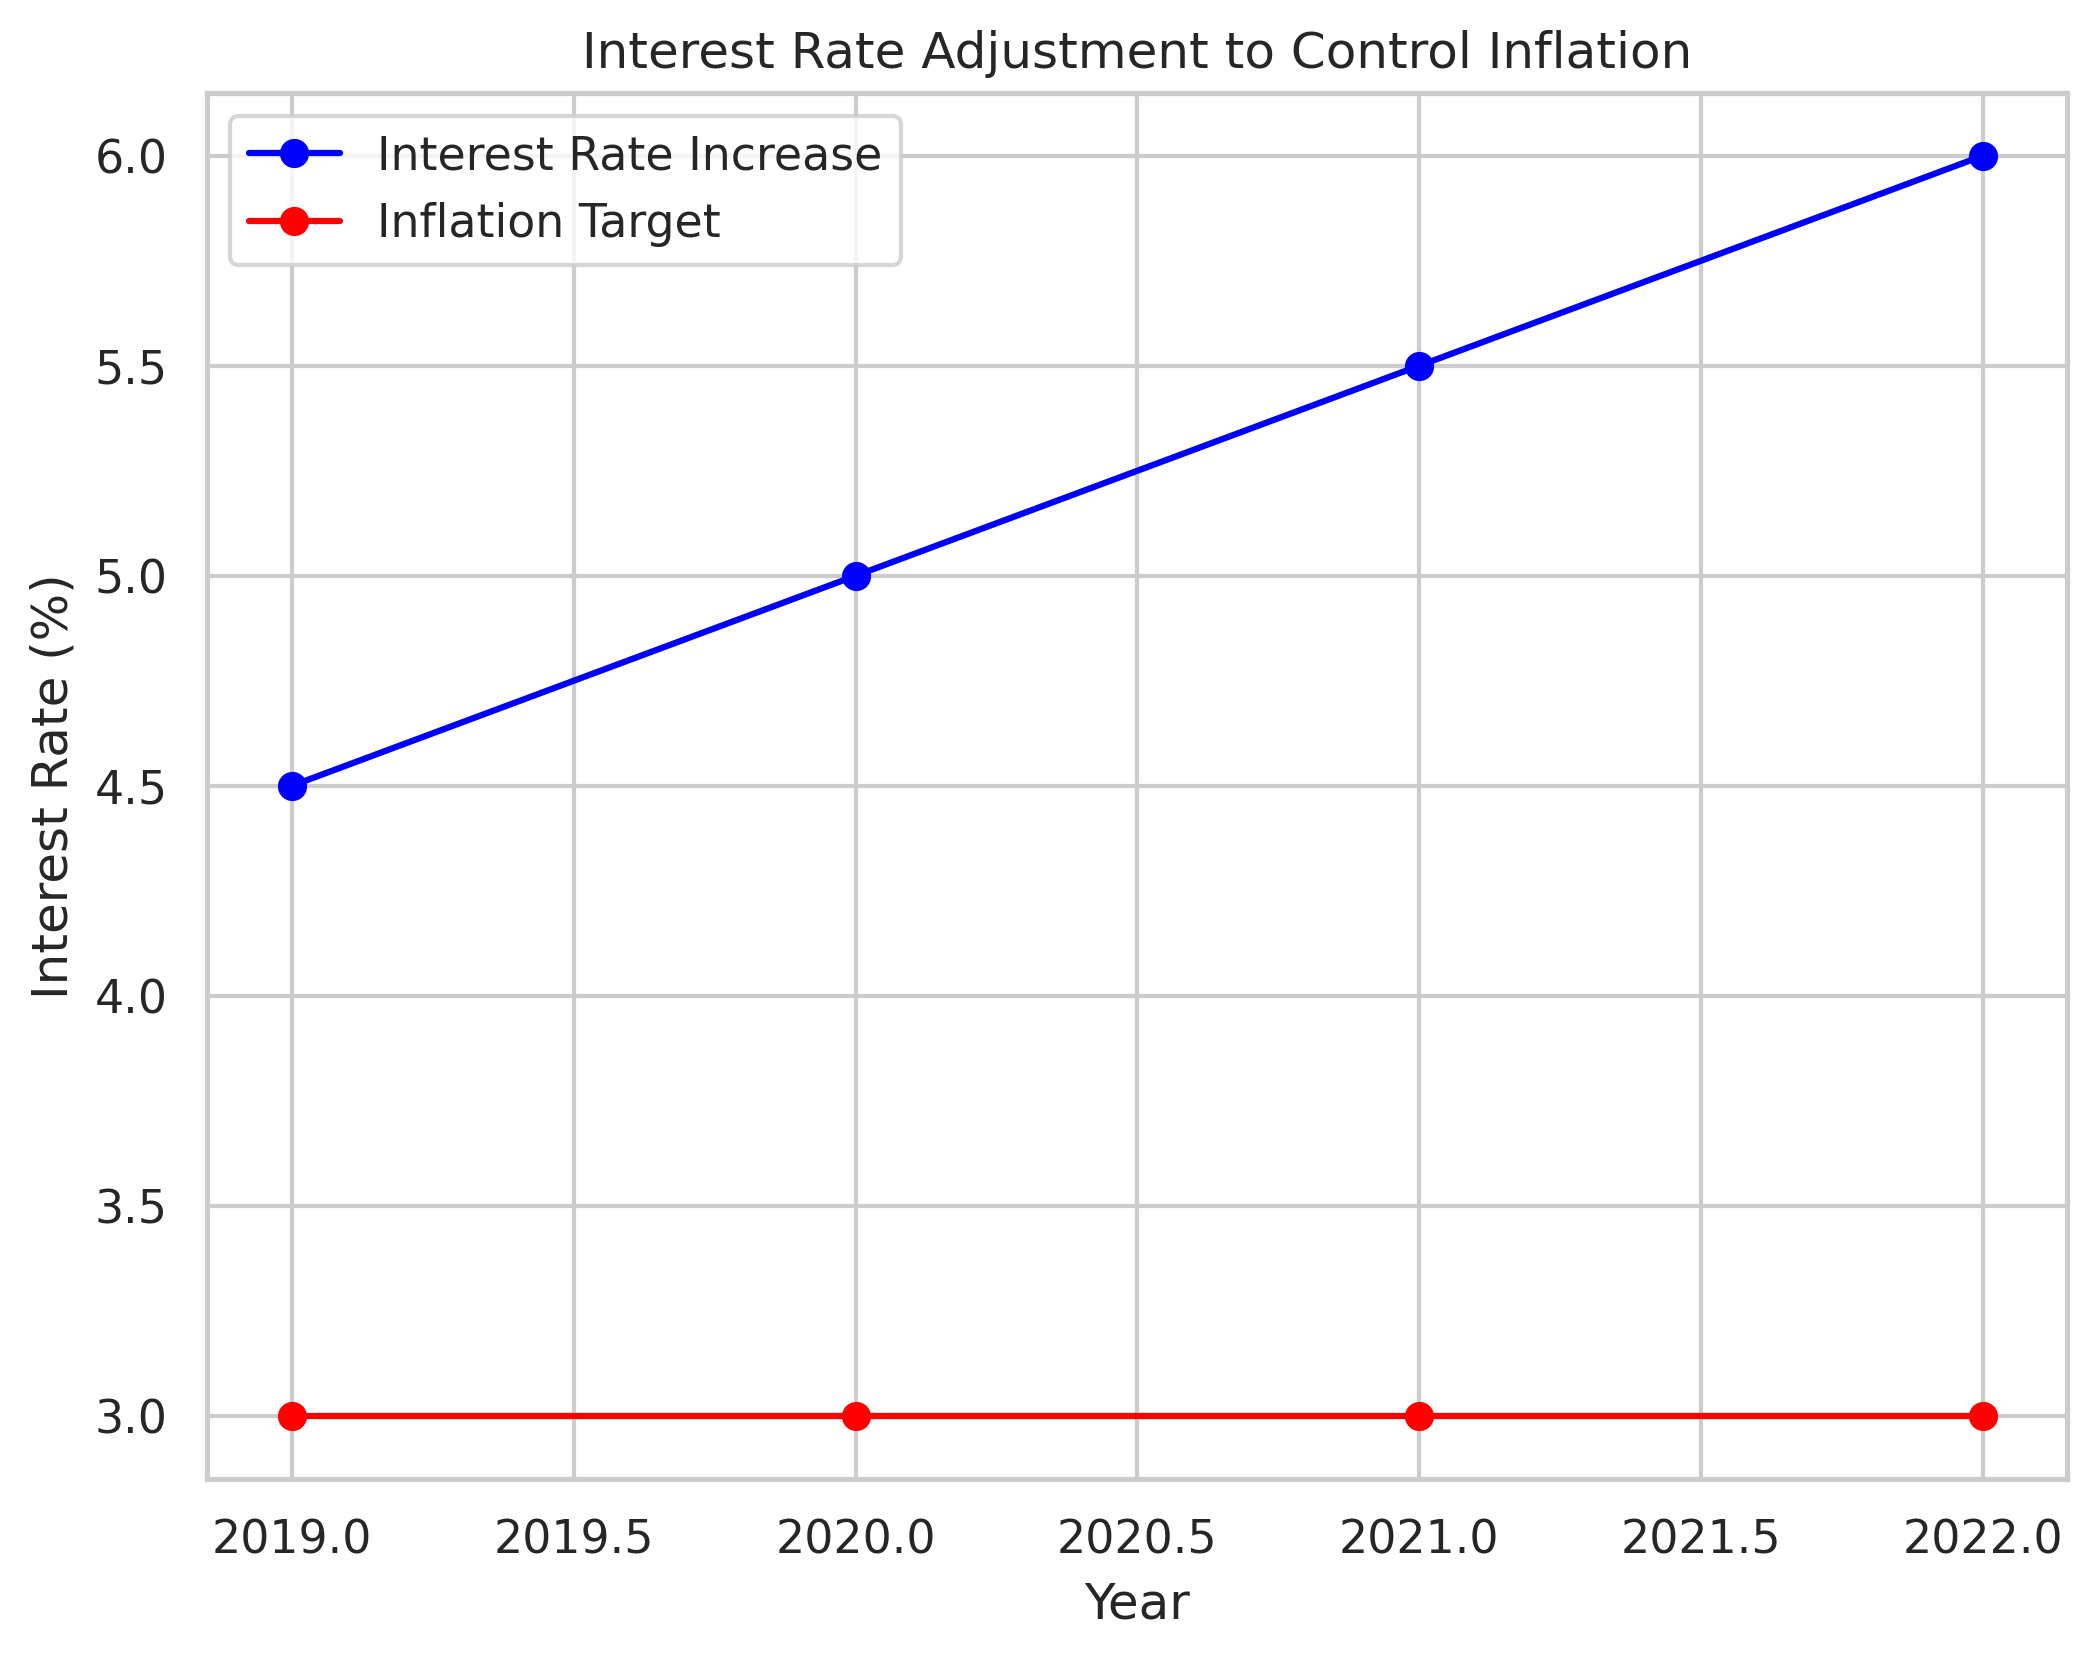
\includegraphics[width=0.53\textwidth]{adjustment.png}
     \caption{Interset Rate Ajustment to Control Inflation}
     \label{fig:graph_1}
\end{figure}

Monetary policy should aim to balance \textbf{\textcolor{teal}{inflation}} and liquidity. While raising \textbf{\textcolor{teal}{interest rates}} 
can help curb inflation, an overly aggressive approach may stifle economic activity and tighten credit conditions. A moderate increase from the current 
\textbf{\textcolor{teal}{4.5\%}} rate could ease inflationary pressures while preserving credit availability. 
Additionally, the Central Bank should introduce a \textbf{\textcolor{teal}{liquidity assistance program}} 
to provide short-term funding for institutions facing deposit outflows, ensuring stability without encouraging
excessive lending. 

Furthermore, targeted \textbf{\textcolor{teal}{open market operations (OMOs)}} should be 
employed to manage liquidity fluctuations. By selectively buying or selling bonds, the Central Bank can regulate
money supply and contain inflation without imposing unnecessary credit constraints \textcolor{orange}{\cite{claessens2017}}.
As shown in Figure 9, a moderate interest rate increase can help align the current rate with the inflation target, 
effectively controlling \textcolor{teal}{\textbf{inflationary pressures}}.

\newpage
\subsection*{Stabilizing the Exchange Rate and Strengthening Foreign Reserves}

\begin{figure}[h]     
     \centering
     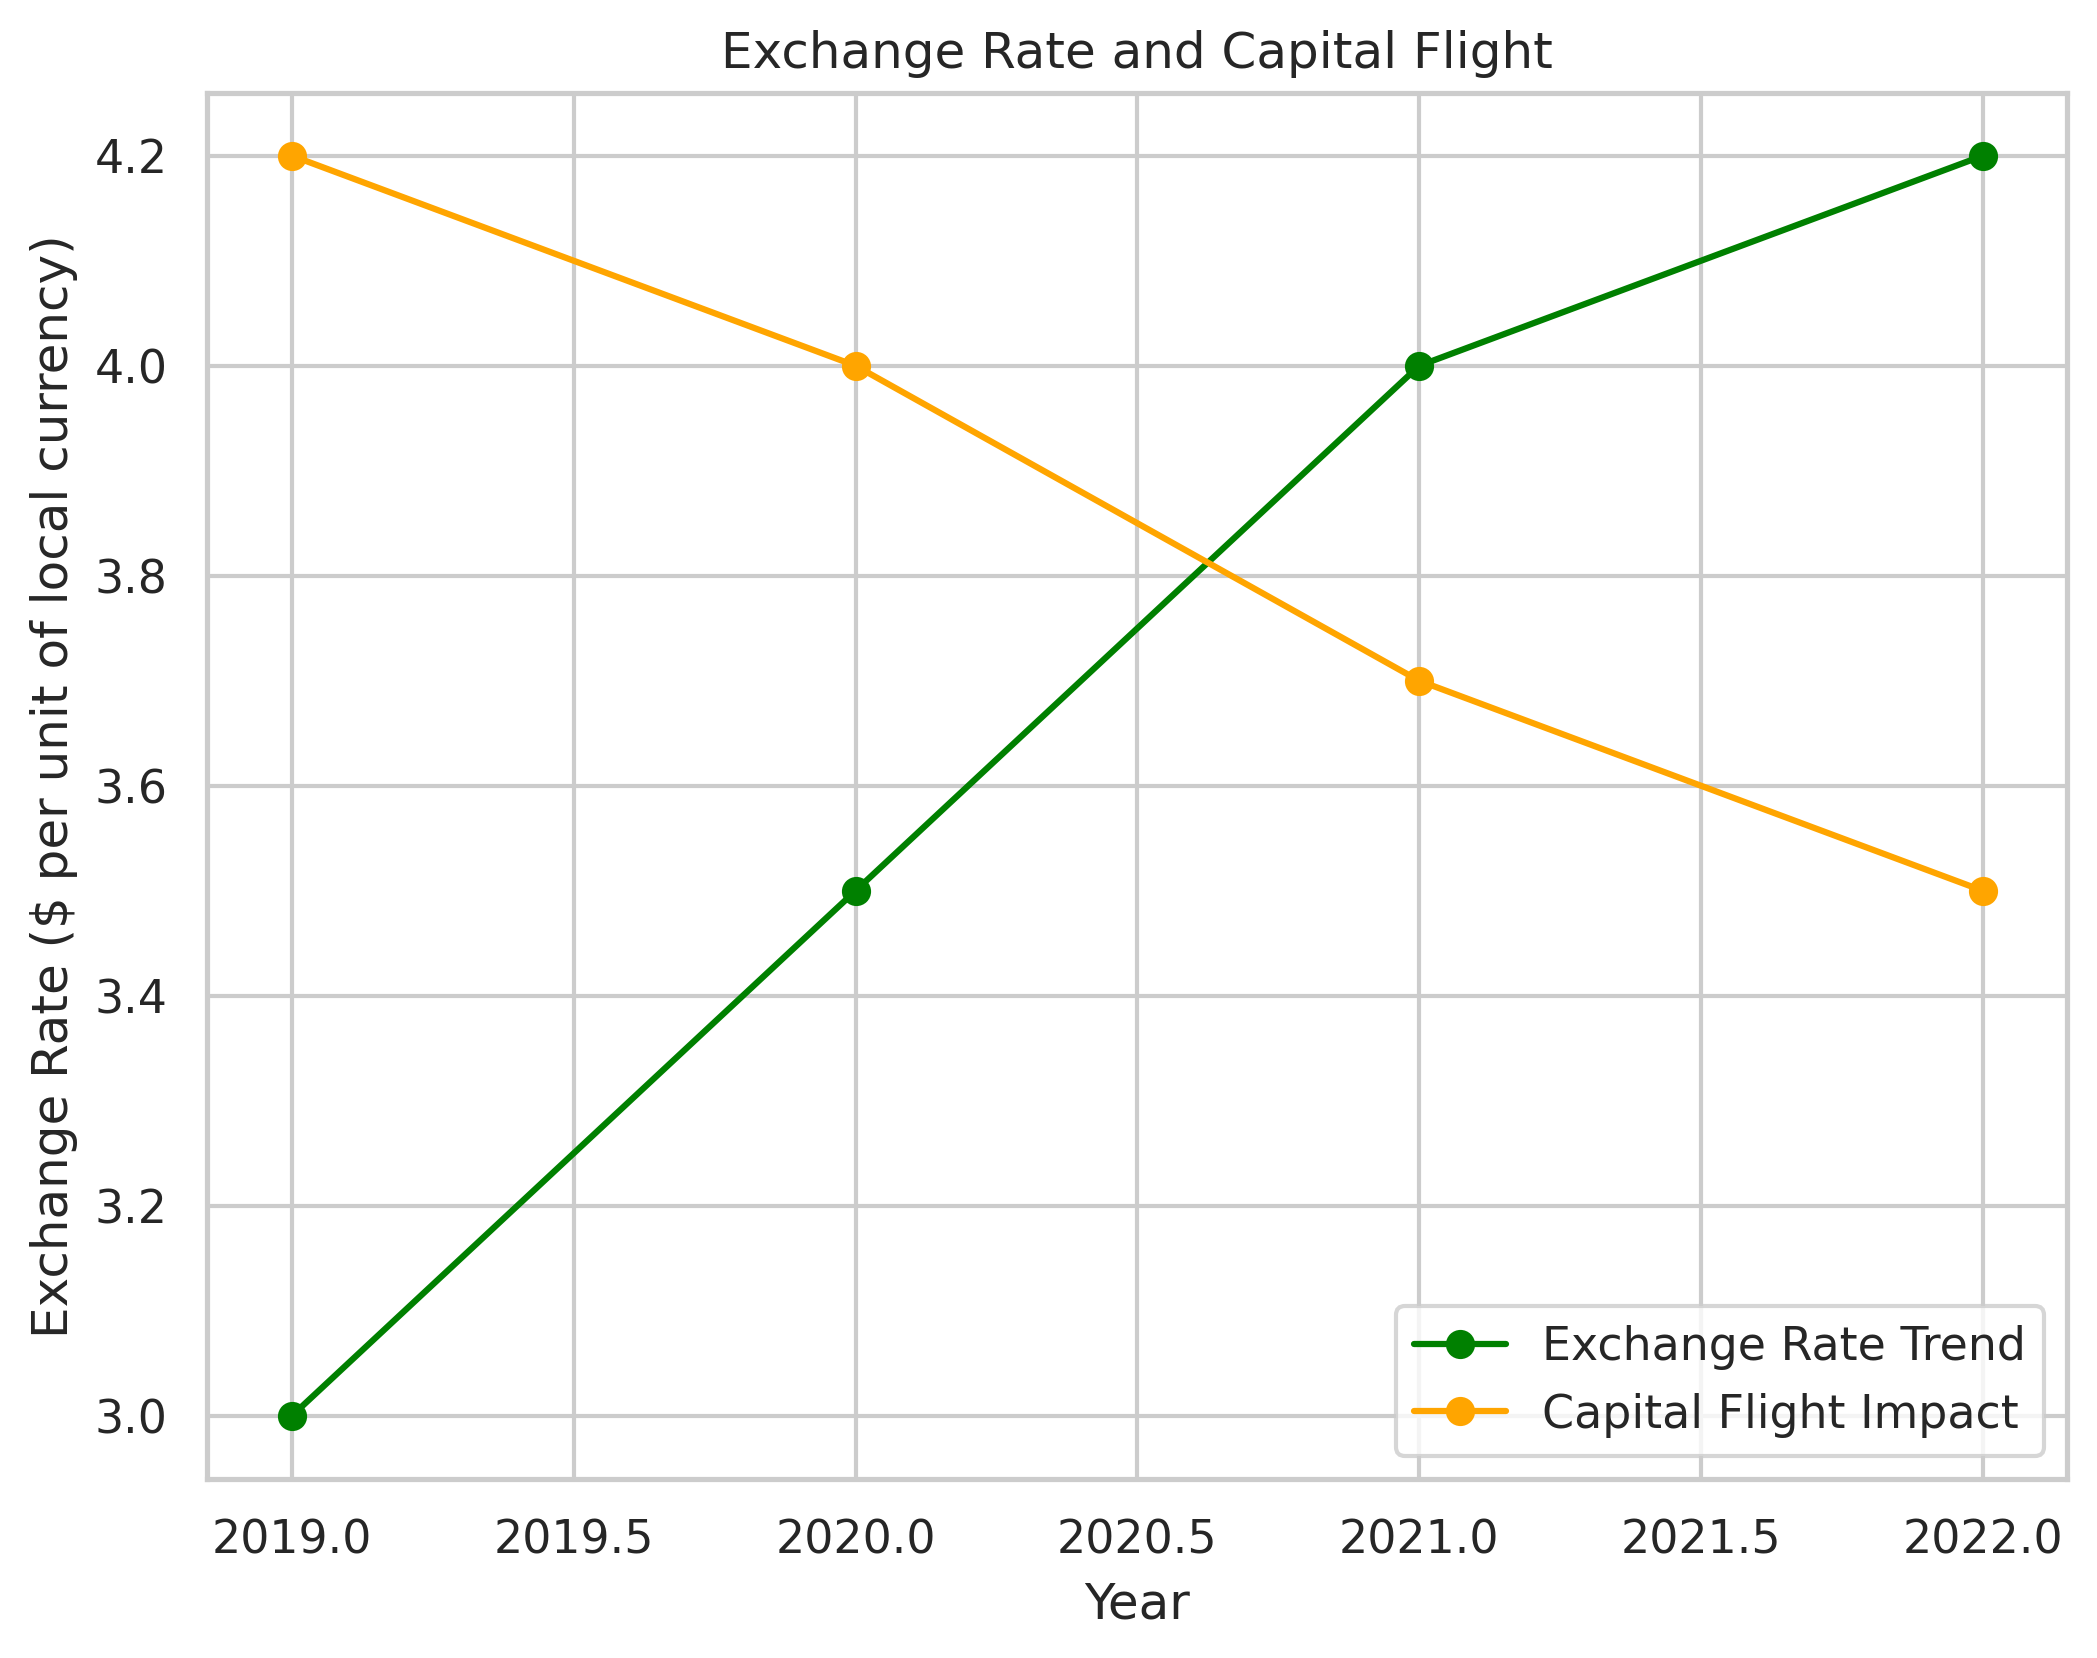
\includegraphics[width=0.53\textwidth]{exchange.png}
     \caption{Exchange Rate and Capital Flight}
     \label{fig:graph_1}
\end{figure}

As depicted in Figure 10, Macaronia's floating exchange rate is under significant
pressure due to \textcolor{teal}{\textbf{capital flight}} and investor withdrawals, 
leading to a rapid depletion of \textcolor{teal}{\textbf{international reserves}}. 
To counter this, the government should engage with the International Monetary Fund (IMF)
to secure a stabilization loan, ensuring that any assistance supports 
\textcolor{teal}{\textbf{long-term economic stability}} rather than providing only short-term 
liquidity relief. Additionally, to rebuild investor confidence, the government should implement 
measured \textcolor{teal}{\textbf{capital controls}} that deter speculative currency outflows while
preserving flexibility for legitimate trade and investment \textcolor{orange}{\cite{imf2024}}.



\subsection*{Strengthening Financial Sector Stability}
Macaronia’s financial sector, particularly commercial banks and credit unions, 
is highly exposed to the \textbf{\textcolor{teal}{real estate market}}, with 
\textbf{\textcolor{teal}{15\%}} and \textbf{\textcolor{teal}{20\%}} of their assets linked to 
\textbf{\textcolor{teal}{Real Estate Investment Trusts (REITs)}}. This concentration has heightened 
systemic risks, especially as REIT values have declined. To mitigate these vulnerabilities, 
the Central Bank should enforce stricter \textbf{\textcolor{teal}{capital adequacy ratios}},
requiring financial institutions to allocate more assets to lower-risk investments
\textcolor{orange}{\cite{mishkin2021}}.


A phased \textbf{\textcolor{teal}{recapitalization process}} should support weaker banks,
incorporating private capital injections, foreign financial assistance, and government-backed stabilization
funds. Furthermore, banks and credit unions should be encouraged to diversify their asset portfolios by
investing in more stable sectors such as \textbf{\textcolor{teal}{manufacturing}},
\textbf{\textcolor{teal}{technology}}, and \textbf{\textcolor{teal}{renewable energy}}. 
Strengthening financial regulations is essential to prevent future crises,
including the creation of an independent financial stability oversight council to monitor systemic risks.
Enhanced transparency and disclosure requirements would further bolster market confidence in financial 
institution \textcolor{orange}{\cite{reinhart2009}}.

\subsection*{Restoring Investor and Depositor Confidence}

\begin{figure}[h]     
     \centering
     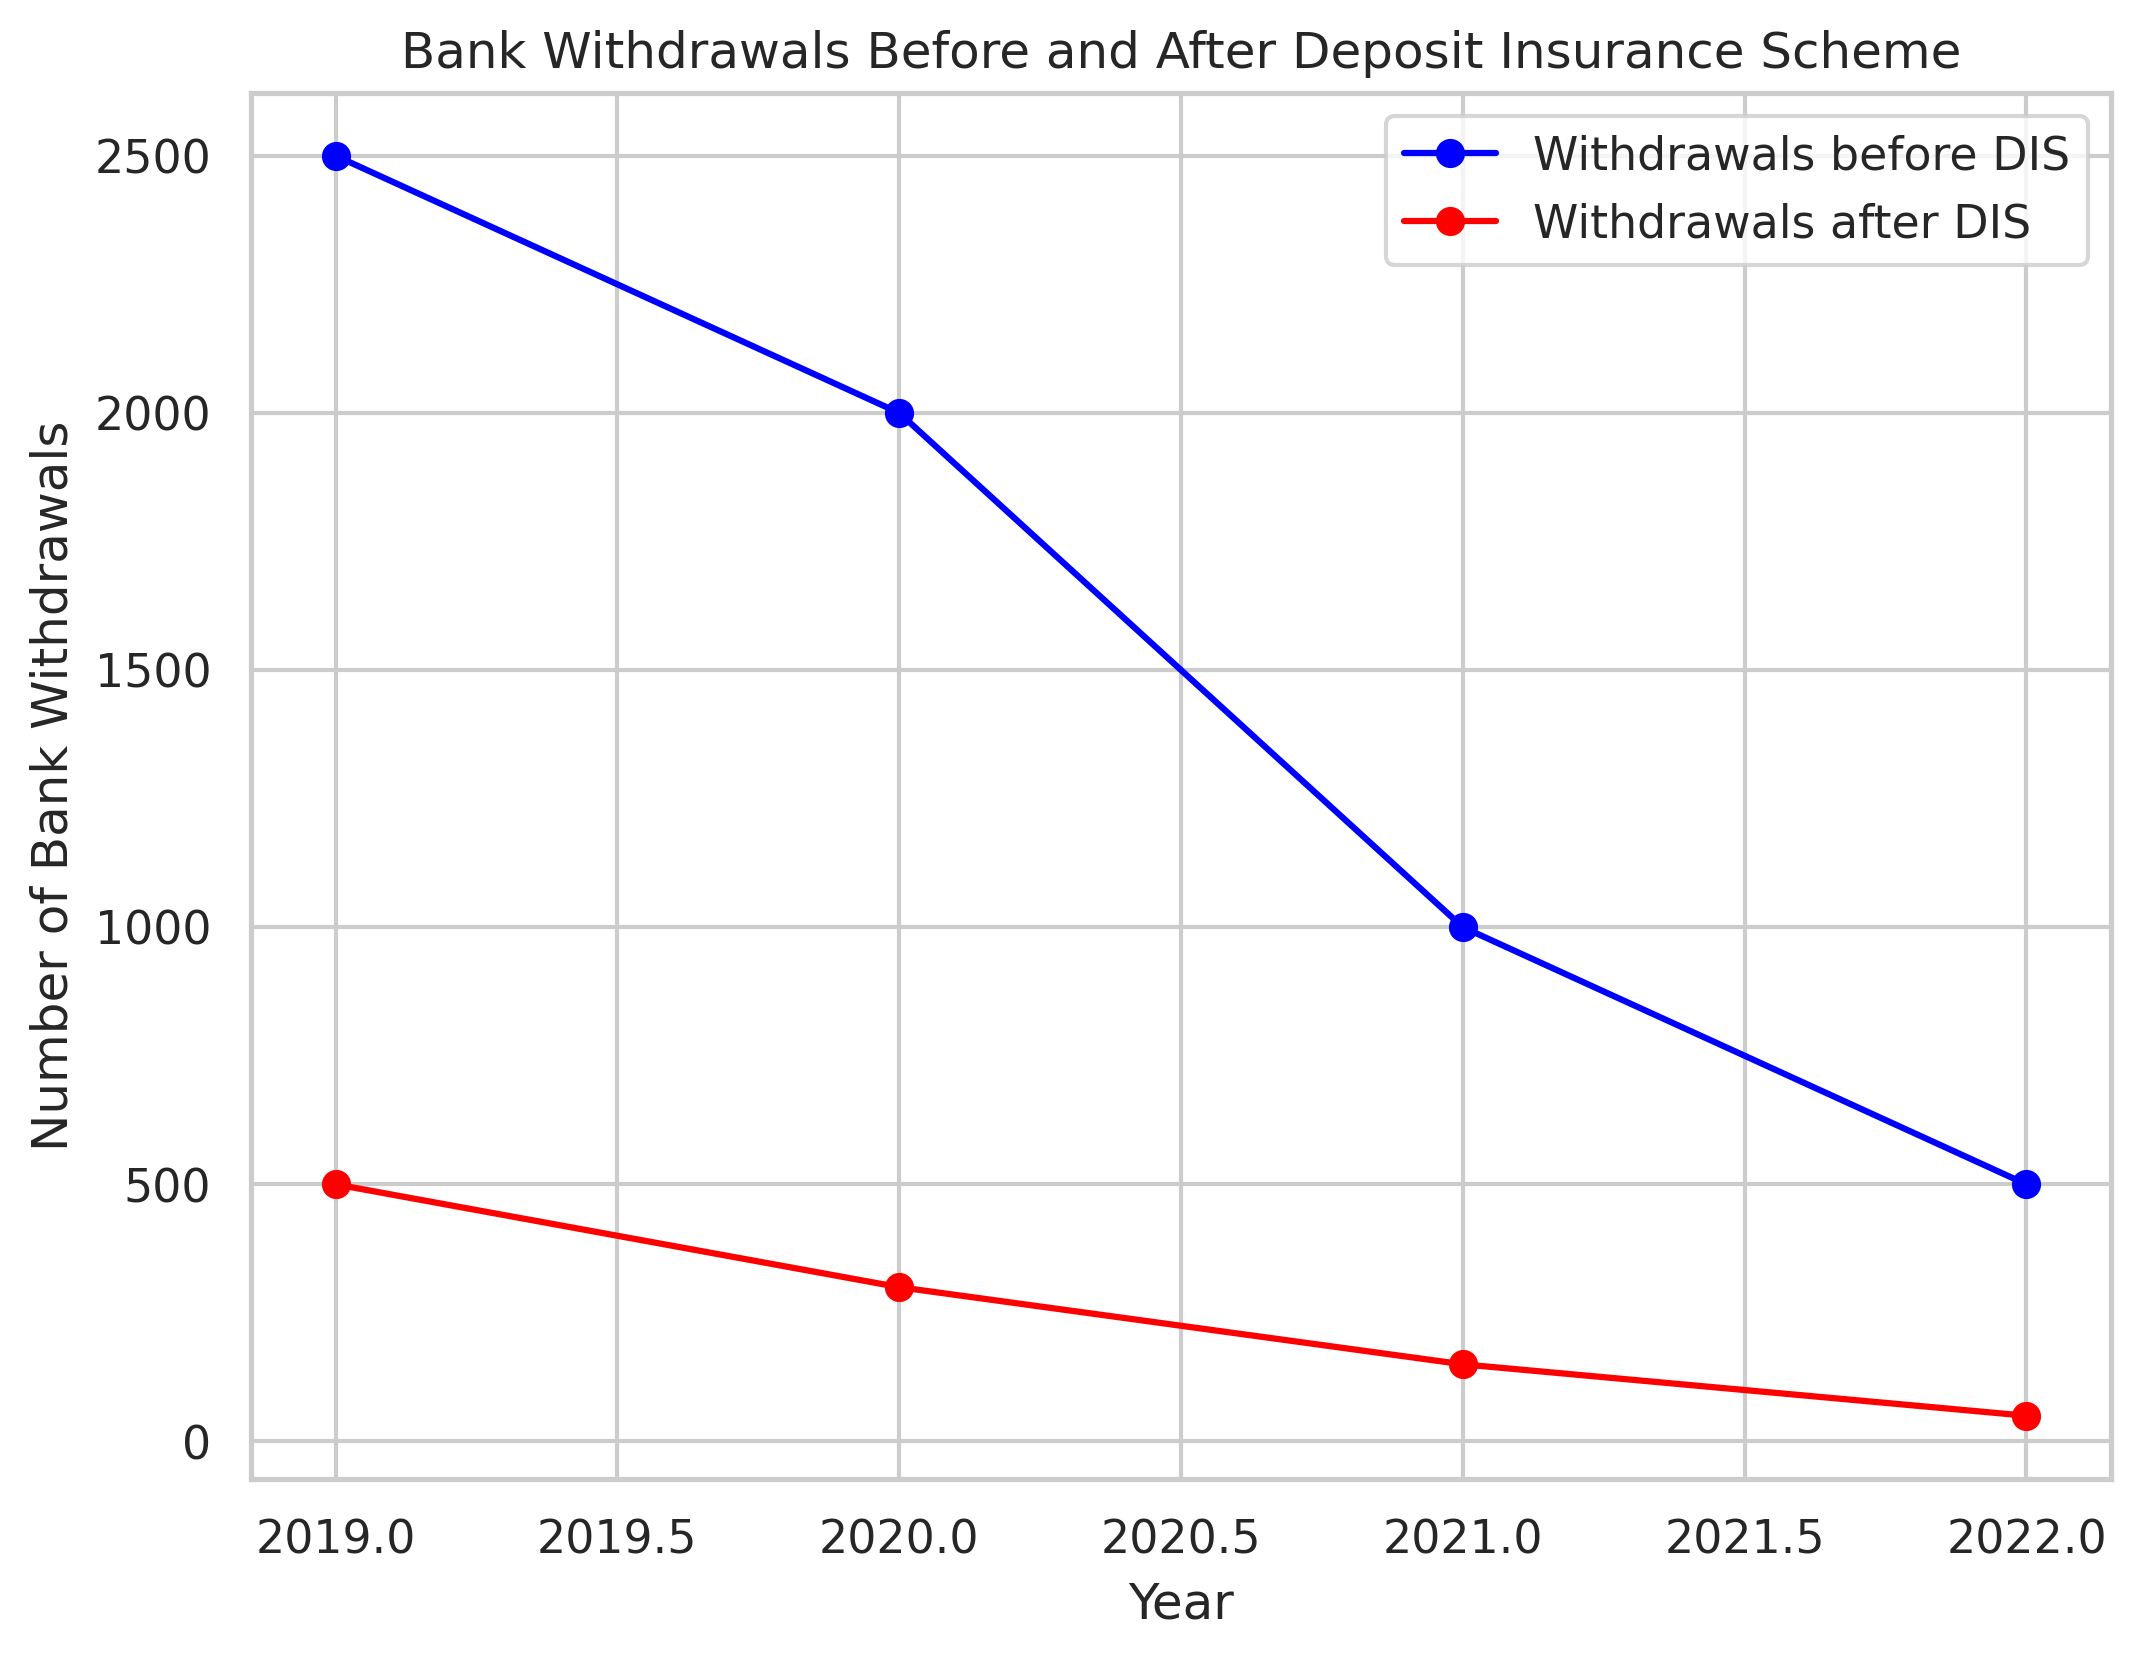
\includegraphics[width=0.53\textwidth]{restore.png}
     \caption{Bank Witdrawals Before And After Deposit Insurance Scheme}
     \label{fig:graph_1}
\end{figure}

Macaronia faces a growing crisis of \textcolor{teal}{\textbf{depositor confidence}}, leading 
to increasing bank withdrawals, a trend evident in Figure 11. The recent collapse of two commercial
banks due to poor capitalization has intensified concerns over \textcolor{teal}{\textbf{financial stability}}.
To address this, the government should introduce a \textcolor{teal}{\textbf{Deposit Insurance Scheme (DIS)}},
which, as Figure 11 suggests, would protect deposits up to a set limit, reducing panic-driven bank runs and 
reassuring depositors of their funds' security. \textcolor{teal}{\textbf{Restoring investor confidence}} is
essential for revitalizing capital inflows into the economy.

To enhance financial transparency,the Central Bank and regulatory authorities 
should regularly publish financial stability reports outlining the state of the
banking sector and ongoing stabilization measures. Additionally, the government
should use tax incentives, investment guarantees, and low-interest loans to attract 
long-term investors. Strengthening investor protection laws and corporate governance will 
further assure both foreign and domestic investors of asset security \textcolor{orange}{\cite{gorton2012}}.

\subsection*{Supporting Financially Excluded and Repressed Households}

The economic downturn has disproportionately affected lower-income households, vulnerable groups, 
and small businesses in Macaronia, limiting access to credit, employment, and essential services.
To mitigate these impacts, the government, should implement targeted 
\textcolor{teal}{\textbf{social protection programs}}, including direct cash transfers to low-income 
households to ensure basic needs are met, subsidized credit programs to support small and medium-sized
businesses, and temporary rent and mortgage relief to prevent widespread foreclosures and homelessness
amid the real estate downturn. As illustrated in Figure 12, a significant portion of the targeted social 
protection programs should be allocated to \textcolor{teal}{\textbf{low-income households}}
(\textcolor{teal}{\textbf{40.0\%}}), followed by \textcolor{teal}{\textbf{financially vulnerable groups}} 
(\textcolor{teal}{\textbf{30.0\%}}) and \textcolor{teal}{\textbf{small businesses}}
(\textcolor{teal}{\textbf{30.0\%}}).


\begin{figure}[h]     
     \centering
     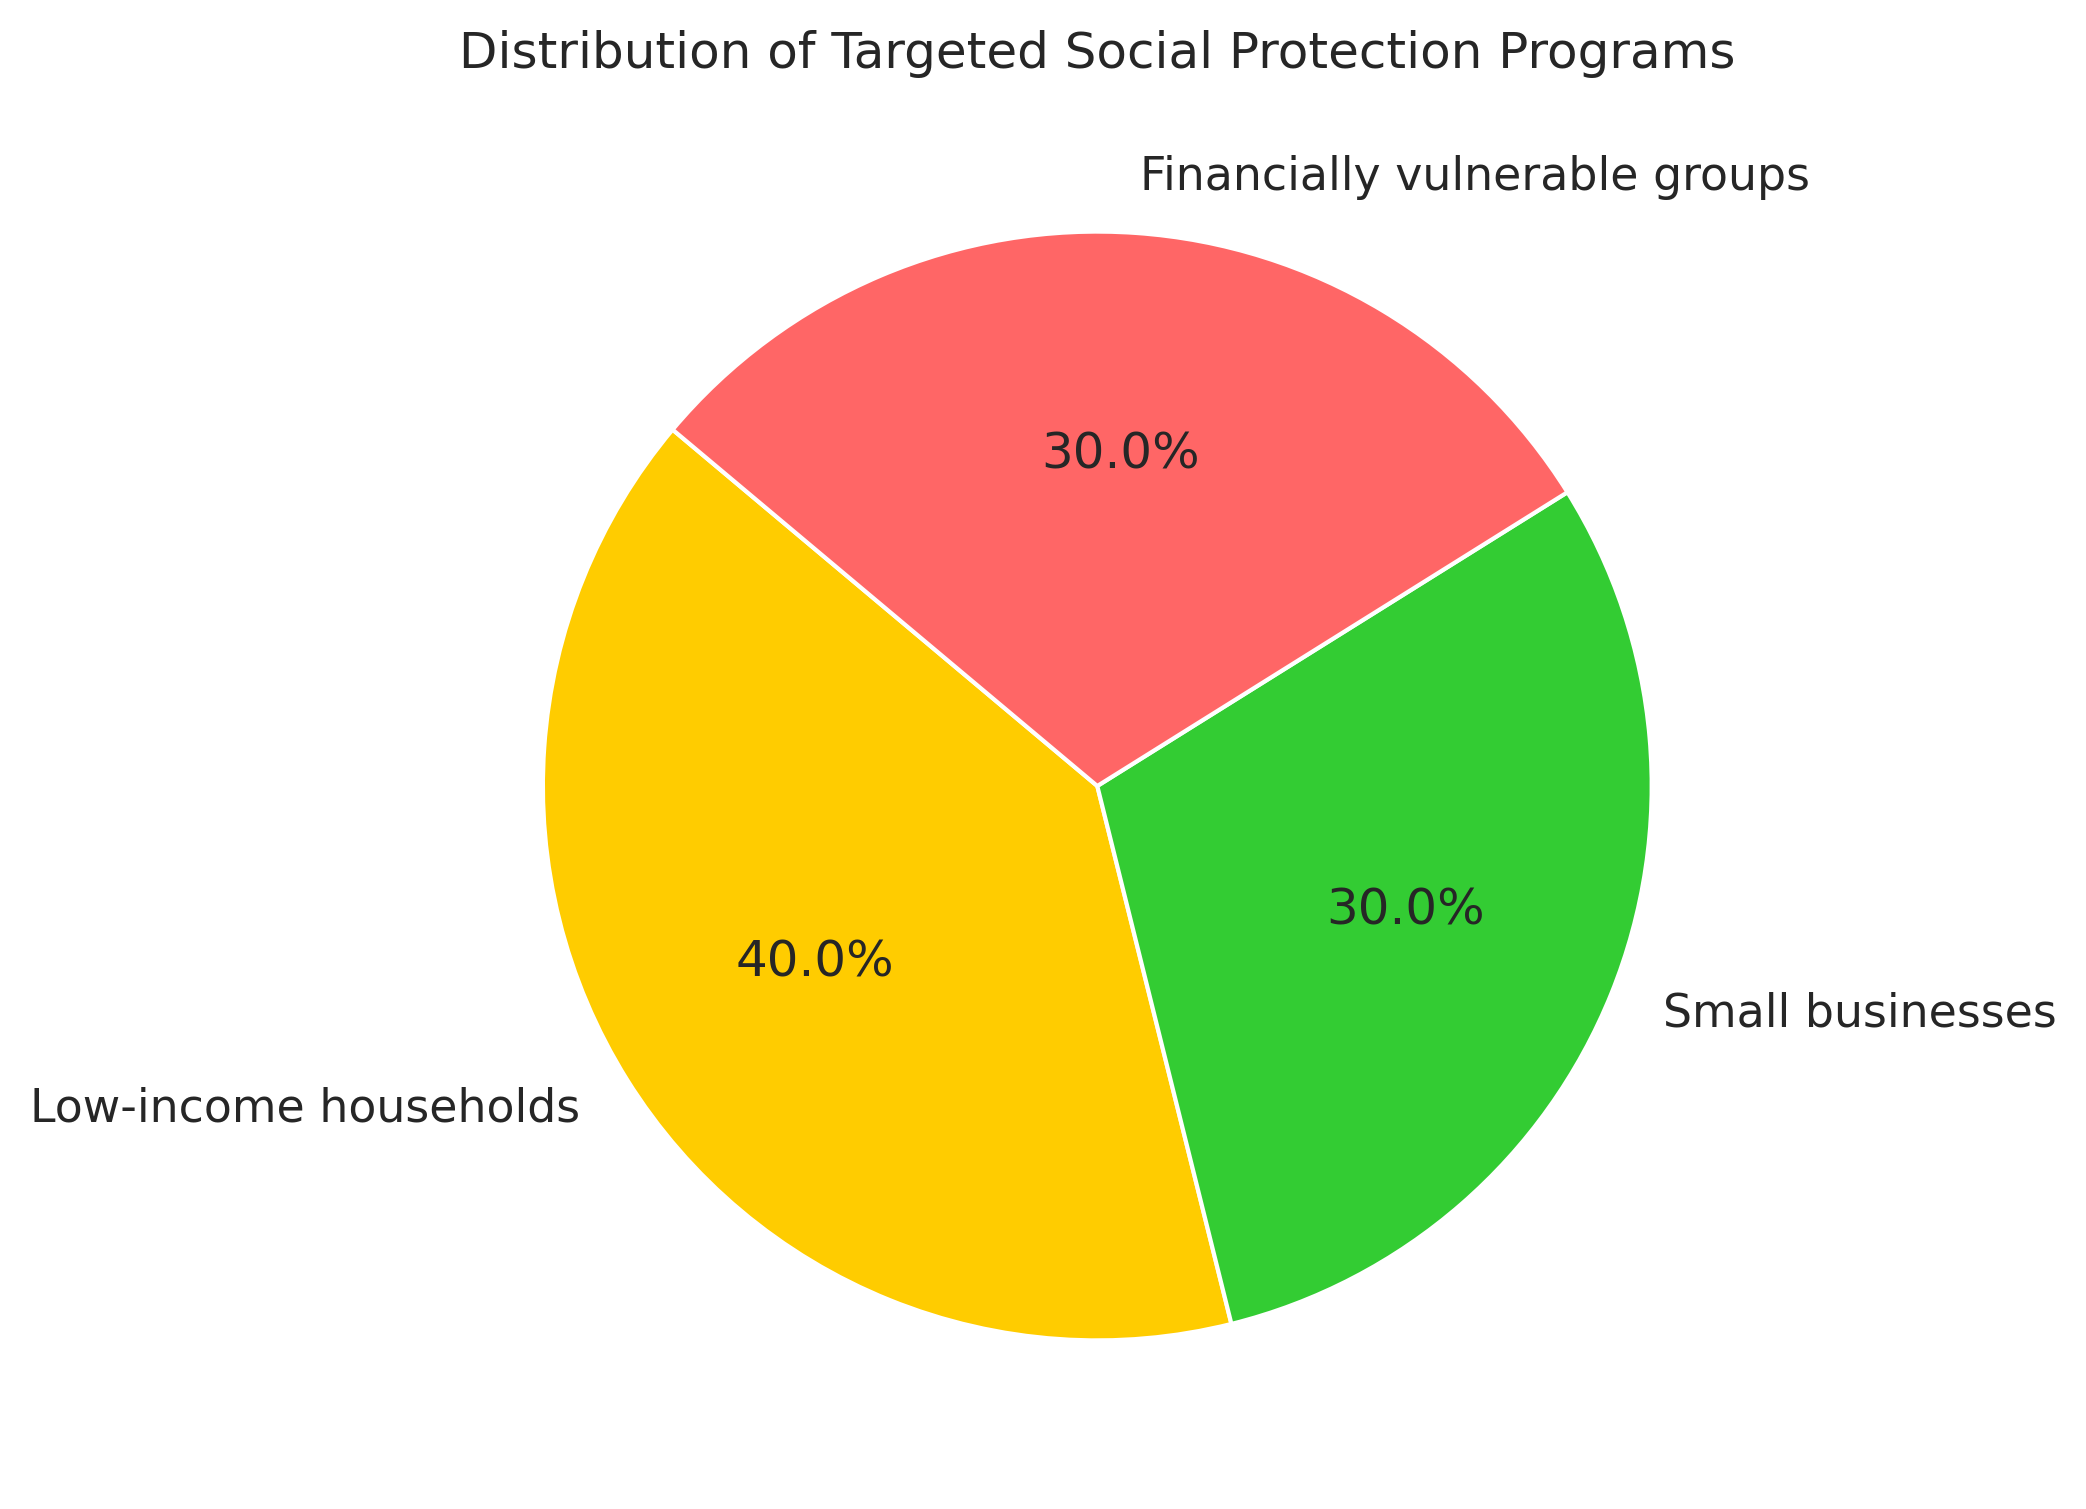
\includegraphics[width=0.53\textwidth]{support.png}
     \caption{Distribution of Targeted Social Platforms}
     \label{fig:graph_1}
\end{figure}

Expanding financial inclusion initiatives will further ensure that 
at-risk populations have access to affordable financial services. Strengthening the 
role of credit unions and microfinance institutions in providing low-interest loans to 
small businesses and individuals will promote economic resilience and stability \textcolor{orange}{\cite{worldbank2023}}.

\subsection*{Promoting Economic Diversification and Long-Term Growth}

\begin{figure}[h]     
     \centering
     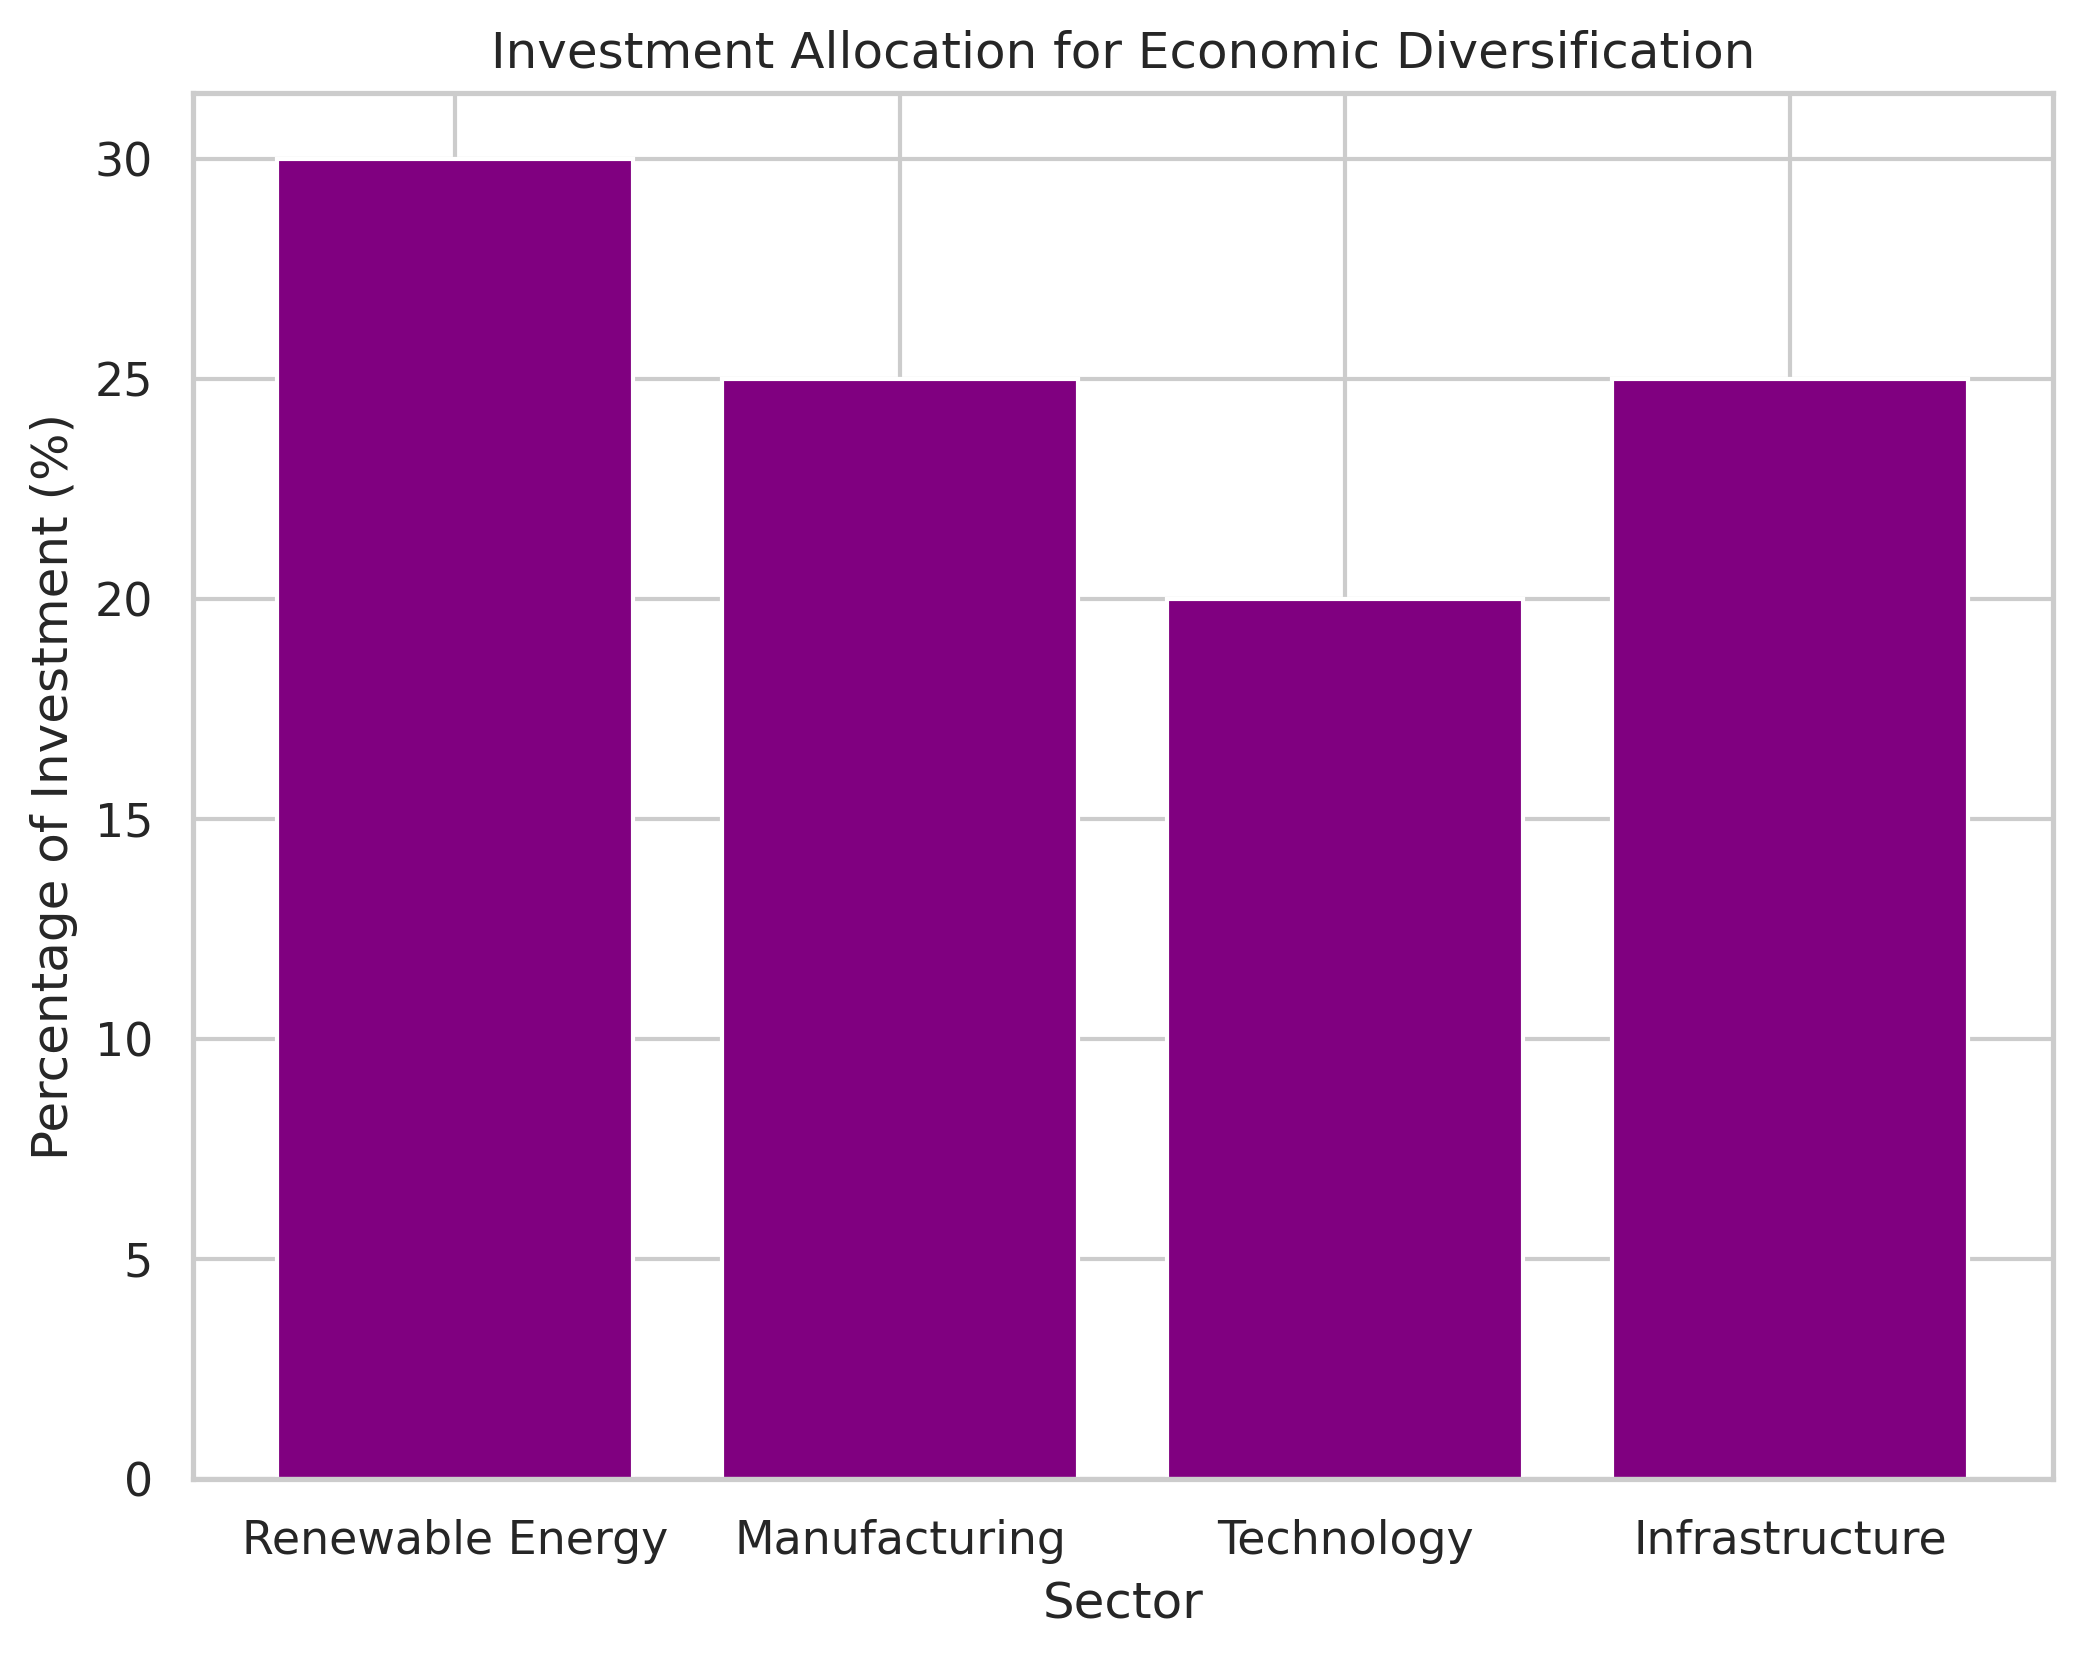
\includegraphics[width=0.53\textwidth]{diversification.png}
     \caption{Investment Allocation for Economic Diversification}
     \label{fig:graph_1}
\end{figure}


Macaronia's economic expansion has been overly reliant on a booming
\textcolor{teal}{\textbf{real estate market}}, which has proven unsustainable.
\textcolor{teal}{\textbf{Diversification}} is essential, and the government should
prioritize domestic economic growth through targeted infrastructure and industrial 
expansion. A key strategy to achieve this is through
\textcolor{teal}{\textbf{Public-Private Partnerships (PPPs)}}, enabling 
collaboration between the private sector and government to develop and manage public
infrastructure. To address logistical bottlenecks and enhance business efficiency, investments
should focus on \textcolor{teal}{\textbf{energy}}, \textcolor{teal}{\textbf{transportation}},
and \textcolor{teal}{\textbf{digital infrastructure}}. As shown in Figure 13, the recommended
investment allocation for economic diversification includes 
\textcolor{teal}{\textbf{Renewable Energy}} (\textcolor{teal}{\textbf{30\%}}),
\textcolor{teal}{\textbf{Manufacturing}} (\textcolor{teal}{\textbf{25\%}}), 
\textcolor{teal}{\textbf{Technology}} (\textcolor{teal}{\textbf{20\%}}), and 
\textcolor{teal}{\textbf{Infrastructure}} (\textcolor{teal}{\textbf{25\%}}). 
Expanding renewable energy, modernizing ports, and improving road networks will boost
competitiveness, attract long-term investment, and reduce import dependency \textcolor{orange}{\cite{engel2014}}.

Given Macaronia's high \textcolor{teal}{\textbf{public debt}} of \textcolor{teal}{\textbf{80\% of GDP}},
direct government-funded projects are financially unfeasible. Utilizing PPPs will allow critical investments
without further straining fiscal deficits. Structuring agreements with risk-sharing mechanisms will ensure 
financial risks are distributed between public and private entities rather than burdening the government alone.
Additionally, infrastructure projects and industrial investments can drive 
\textcolor{teal}{\textbf{job creation}} and \textcolor{teal}{\textbf{economic inclusion}}, 
particularly for low-income and financially marginalized populations. Encouraging private sector
participation in vocational training programs will help develop a skilled workforce to support
diversified economic growth. Strengthening public-private partnerships will ensure that economic
expansion is not overly reliant on foreign capital inflows \textcolor{orange}{\cite{bernanke2013}}.
